% =====================================================================
% Semana 1 · S1.6 — Potenciómetro y efecto de carga
% Fundamentos de Sistemas Electrónicos Analógicos (Ingeniería Aeroespacial)
% Compilar: pdflatex semana_1_s16_divisor_cargado.tex  (2 pasadas)
% =====================================================================
\documentclass[aspectratio=169]{beamer}

\usepackage[utf8]{inputenc}
\usepackage[T1]{fontenc}
\usepackage{lmodern}
\usepackage[spanish,es-tabla]{babel}
\usepackage{amsmath,amssymb}
\usepackage{siunitx}
\usepackage{booktabs}
\usepackage{microtype}
\usepackage{circuitikz}

\definecolor{navy}{RGB}{23,54,93}
\definecolor{navysoft}{RGB}{72,101,140}
\definecolor{gold}{RGB}{179,142,62}
\definecolor{ink}{RGB}{44,51,58}
\definecolor{soft}{RGB}{244,241,234}

\usetheme{default}
\setbeamertemplate{navigation symbols}{}
\setbeamertemplate{footline}[frame number]
\setbeamercolor{structure}{fg=navy}
\setbeamercolor{frametitle}{fg=white,bg=navy}
\setbeamercolor{title}{fg=navy}
\setbeamercolor{subtitle}{fg=navysoft}
\setbeamercolor{itemize item}{fg=gold}
\setbeamercolor{itemize subitem}{fg=gold}
\setbeamercolor{block title}{fg=white,bg=navy}
\setbeamercolor{block body}{bg=soft}
\setbeamercolor{example text}{fg=navy}
\setbeamertemplate{itemize item}{\scriptsize\raise1.25pt\hbox{\donotcoloroutermaths$\bullet$}}
\setbeamertemplate{itemize subitem}{\scriptsize\raise1.25pt\hbox{\donotcoloroutermaths$\circ$}}
\setbeamerfont{frametitle}{size=\large,series=\bfseries}

\title[S1.6 · Divisor cargado]{Potenciómetro y efecto de carga}
\subtitle{S1.6 — Simulaciones y laboratorio de la Semana 1}
\institute{Licenciatura en Ingeniería Aeroespacial\\ UNAM · ENES Unidad Juriquilla}
\author{M. en C. José de Jesús Santana Ramírez}
\date{Semestre 2027-1}

\begin{document}

% ---------------------------------------------------------------------
\begin{frame}[plain]
  \titlepage
\end{frame}

% ---------------------------------------------------------------------
\begin{frame}{Objetivos de la sesión}
  \begin{itemize}
    \item Modelar un \textbf{potenciómetro} como divisor de tensión con cursor ($\alpha$).
    \item Distinguir \textbf{divisor sin carga} ($V_{out} = V_{in}\,\alpha$) de \textbf{divisor cargado}.
    \item Calcular el \textbf{efecto de carga} con $R_L = 10\,\text{k}\Omega$ (igual al pot).
    \item Responder la pregunta de cierre: \emph{¿cuándo un divisor es ``fuente ideal'' y cuándo necesita un buffer?}
  \end{itemize}
  \pause
  \begin{block}{Pregunta inicial}
    ¿Cuánto se equivoca la salida de un potenciómetro de 10 k$\Omega$ cuando se le conecta una carga de 10 k$\Omega$?
  \end{block}
\end{frame}

% ---------------------------------------------------------------------
\begin{frame}{Teoría 1 · Potenciómetro como divisor}
  Un potenciómetro lineal de valor $R_{pot}$ con cursor en fracción $\alpha$ se
  modela como dos resistencias:
  \[
    R_{top} = R_{pot}\,(1-\alpha)
    \qquad\qquad
    R_{bot} = R_{pot}\,\alpha
    \qquad (0 \le \alpha \le 1)
  \]
  \begin{center}
    \begin{circuitikz}[american voltages, scale=0.9]
      \draw (0,3) to[V, l={$V_{in}$}, i=$I$] (0,0);
      \draw (0,3) -- (1.2,3) to[R, l={$R_{top}$}] (4.2,3);
      \draw (4.2,3) -- (5.4,3) to[R, l={$R_{bot}$}] (5.4,0);
      \draw (5.4,0) -- (0,0);
      \node[circle, fill=gold, inner sep=0.9pt] at (4.2,3) {};
      \node[above, text=gold] at (4.2,3.28) {$V_{out}$};
    \node[ground] at (0,0) {};
    \end{circuitikz}
  \end{center}
  \pause
  \begin{itemize}
    \item Sin carga conectada, solo circula la corriente del propio divisor.
  \end{itemize}
\end{frame}

% ---------------------------------------------------------------------
\begin{frame}{Teoría 2 · Divisor sin carga (ideal)}
  Por el divisor de tensión de S1.2:
  \[
    V_{out}^{ideal} = V_{in}\cdot\frac{R_{bot}}{R_{top}+R_{bot}}
    = V_{in}\cdot\frac{R_{pot}\,\alpha}{R_{pot}}
    = V_{in}\,\alpha
  \]
  \pause
  \begin{itemize}
    \item Salida \textbf{lineal} con la posición del cursor: la ``curva'' esperada del potenciómetro.
    \item Con $V_{in} = 5$ V: a 10\,\% $\rightarrow$ 0.5 V; a 50\,\% $\rightarrow$ 2.5 V; a 90\,\% $\rightarrow$ 4.5 V.
    \item Este es el comportamiento que se asume cuando se dice ``el potenciómetro divide''.
  \end{itemize}
\end{frame}

% ---------------------------------------------------------------------
\begin{frame}{Teoría 3 · Divisor cargado: el efecto de carga}
  Si se conecta una carga $R_L$ a la salida, $R_L$ queda \textbf{en paralelo con} $R_{bot}$:
  \[
    V_{out}^{cargada} = V_{in}\cdot\frac{R_{bot}\parallel R_L}{R_{top} + (R_{bot}\parallel R_L)}
    \qquad\text{con}\quad
    R_{bot}\parallel R_L = \frac{R_{bot}\,R_L}{R_{bot}+R_L}
  \]
  \pause
  \begin{itemize}
    \item Como $R_{bot}\parallel R_L < R_{bot}$, la salida \textbf{cae} respecto del caso ideal.
    \item El divisor se comporta como una fuente con \textbf{impedancia de salida}
      $Z_{out} = R_{top}\parallel R_{bot}$ (máximo $R_{pot}/4$ en el centro).
    \item Si $R_L \gg Z_{out}$, el efecto es despreciable; si $R_L \approx R_{pot}$, no.
  \end{itemize}
\end{frame}

% ---------------------------------------------------------------------
\begin{frame}{Ejercicio · Enunciado}
  \begin{block}{Pot de 10 k$\Omega$ sobre 5 V, cargado con 10 k$\Omega$}
    \centering
    $V_{in} = \SI{5}{\volt}$, \quad $R_{pot} = \SI{10}{\kilo\ohm}$, \quad $R_L = \SI{10}{\kilo\ohm}$.
  \end{block}
  \begin{center}
    \begin{circuitikz}[american voltages, scale=0.9]
      \draw (0,3) to[V, l={$V_{in}=5\,\mathrm{V}$}, i=$I$] (0,0);
      \draw (0,3) -- (1.2,3) to[R, l={$R_{top}$}] (4.2,3);
      \draw (4.2,3) -- (4.9,3) to[R, l={$R_{bot}$}] (4.9,0);
      \draw (4.9,3) -- (6.4,3) to[R, l={$R_{L}$}] (6.4,0);
      \draw (6.4,0) -- (0,0);
    \node[ground] at (0,0) {};
    \end{circuitikz}
  \end{center}
  \textbf{Determinar:} $V_{out}^{ideal}$ y $V_{out}^{cargada}$ en posiciones
  $\alpha = 0.1$, $0.5$ y $0.9$, y el error porcentual.
\end{frame}

% ---------------------------------------------------------------------
\begin{frame}{Desarrollo · Paso 1 — $\alpha = 0.1$ (cursor al 10\,\%)}
  \[
    R_{top} = 9\,\text{k}\Omega,\quad R_{bot} = 1\,\text{k}\Omega
    \qquad\Rightarrow\qquad
    V_{out}^{ideal} = 5\cdot 0.1 = \SI{0.500}{\volt}
  \]
  \[
    R_{bot}\parallel R_L = \frac{1\cdot 10}{11}\,\text{k}\Omega = \SI{909.1}{\ohm}
    \qquad
    V_{out}^{cargada} = 5\cdot\frac{909.1}{9000+909.1} = \SI{0.459}{\volt}
  \]
  \[
    \text{error} = \frac{0.500-0.459}{0.500} = \SI{8.3}{\percent}
  \]
  \pause
  \begin{itemize}
    \item La carga ``roba'' corriente y la salida cae casi medio voltio por debajo de lo esperado.
  \end{itemize}
\end{frame}

% ---------------------------------------------------------------------
\begin{frame}{Desarrollo · Paso 2 — $\alpha = 0.5$ (centro)}
  \[
    R_{top} = R_{bot} = 5\,\text{k}\Omega
    \qquad\Rightarrow\qquad
    V_{out}^{ideal} = 5\cdot 0.5 = \SI{2.500}{\volt}
  \]
  \[
    R_{bot}\parallel R_L = \frac{5\cdot 10}{15}\,\text{k}\Omega = \SI{3.333}{\kilo\ohm}
    \qquad
    V_{out}^{cargada} = 5\cdot\frac{3.333}{5+3.333} = \SI{2.000}{\volt}
  \]
  \[
    \text{error} = \frac{2.500-2.000}{2.500} = \SI{20}{\percent}
  \]
  \pause
  \begin{alertblock}{Punto de mayor error}
    En el centro la impedancia de salida del divisor es máxima
    ($Z_{out} = 2.5\,\text{k}\Omega$) y el error de carga alcanza el \textbf{20\,\%}.
  \end{alertblock}
\end{frame}

% ---------------------------------------------------------------------
\begin{frame}{Desarrollo · Paso 3 — $\alpha = 0.9$ (cursor al 90\,\%)}
  \[
    R_{top} = 1\,\text{k}\Omega,\quad R_{bot} = 9\,\text{k}\Omega
    \qquad\Rightarrow\qquad
    V_{out}^{ideal} = 5\cdot 0.9 = \SI{4.500}{\volt}
  \]
  \[
    R_{bot}\parallel R_L = \frac{9\cdot 10}{19}\,\text{k}\Omega = \SI{4.737}{\kilo\ohm}
    \qquad
    V_{out}^{cargada} = 5\cdot\frac{4.737}{1+4.737} = \SI{4.128}{\volt}
  \]
  \[
    \text{error} = \frac{4.500-4.128}{4.500} = \SI{8.3}{\percent}
  \]
  \pause
  \begin{itemize}
    \item El error vuelve a caer al 8.3\,\%: el efecto de carga es \textbf{máximo en el centro}.
  \end{itemize}
\end{frame}

% ---------------------------------------------------------------------
\begin{frame}{Desarrollo · Paso 4 — Tabla resumen}
  \begin{table}
    \small
    \begin{tabular}{lccc}
      \toprule
      Posición $\alpha$ & $V_{out}^{ideal}$ & $V_{out}^{cargada}$ & Error \\
      \midrule
      10\,\% & \SI{0.500}{\volt} & \SI{0.459}{\volt} & \SI{8.3}{\percent} \\
      50\,\% & \SI{2.500}{\volt} & \SI{2.000}{\volt} & \textbf{\SI{20}{\percent}} \\
      90\,\% & \SI{4.500}{\volt} & \SI{4.128}{\volt} & \SI{8.3}{\percent} \\
      \bottomrule
    \end{tabular}
  \end{table}
  \pause
  \begin{block}{Conclusión de diseño}
    Con $R_L = R_{pot}$ el divisor \textbf{no se comporta como fuente ideal}: el
    error llega al 20\,\% en el centro. Regla práctica: necesitas $R_L \ge 10\cdot Z_{out}$
    para error $\lesssim 5\,\text{\%}$, o bien un \textbf{buffer} (seguidor de emisor/op-amp).
  \end{block}
\end{frame}

% ---------------------------------------------------------------------
\begin{frame}[fragile]{Verificación en LTspice}
  Abrir \texttt{semana1\_06\_divisor\_cargado.asc} (dos ramas: sin carga
  \texttt{vout\_u} y cargada \texttt{vout\_l}, barriendo $\alpha$ de 0.1 a 0.9)
  y consultar el Error Log:

  \begin{verbatim}
.meas dc V_unloaded_10pct FIND V(vout_u) AT=0.1
.meas dc V_loaded_10pct   FIND V(vout_l) AT=0.1
.meas dc V_unloaded_50pct FIND V(vout_u) AT=0.5
.meas dc V_loaded_50pct   FIND V(vout_l) AT=0.5
  \end{verbatim}

  \textbf{Criterio de éxito:} en el centro, $V(vout_u) \approx \SI{2.5}{\volt}$ y
  $V(vout_l) \approx \SI{2.0}{\volt}$ (error del 20\,\%).
\end{frame}

% ---------------------------------------------------------------------
  % ---------------------------------------------------------------------
  \begin{frame}{Resultado de la simulación}
    \begin{center}
      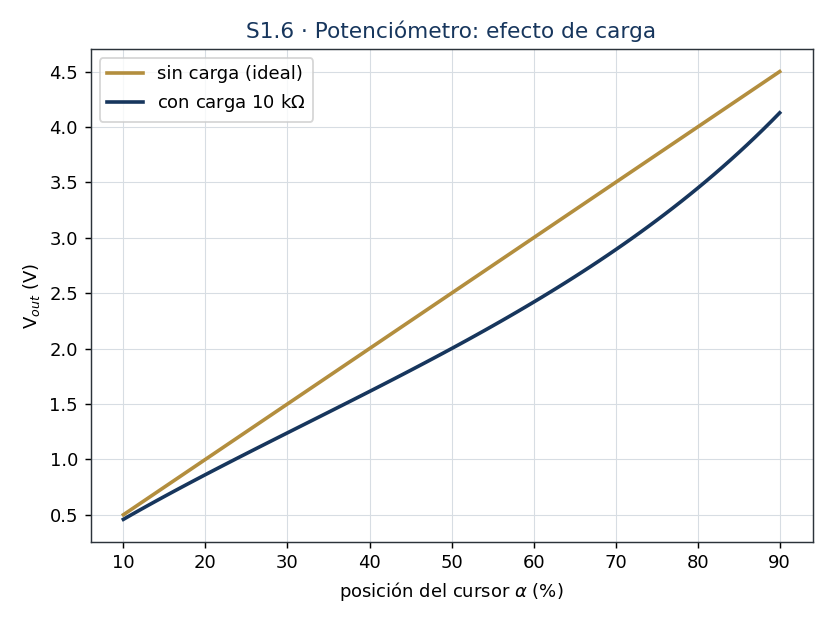
\includegraphics[width=0.78\textwidth]{figs/s16_pot.png}
    \end{center}
    \begin{itemize}
      \item La carga de 10 k$\Omega$ hace que la salida caiga hasta 20\% en el centro.
    \end{itemize}
  \end{frame}

  % ---------------------------------------------------------------------
  \begin{frame}{Errores comunes}
  \begin{table}
    \small
    \begin{tabular}{p{0.34\textwidth}p{0.30\textwidth}p{0.30\textwidth}}
      \toprule
      Error & Consecuencia & Corrección \\
      \midrule
      Ignorar $R_L$ al calcular el divisor & Salida sobreestimada & Paralelar $R_{bot}$ con $R_L$ \\
      Suponer $V_{out} = V_{in}\,\alpha$ siempre & Error de hasta 20\,\% & Verificar $R_L \gg Z_{out}$ \\
      No considerar la impedancia del ADC & Conversión errónea & Buffer + capacitor \\
      Usar trimpot sin fijar en vibración & Calibración que se mueve & Fijar con epoxi o red de precisión \\
      \bottomrule
    \end{tabular}
  \end{table}
\end{frame}

% ---------------------------------------------------------------------
\begin{frame}{Lectura aeroespacial}
  \begin{itemize}
    \item \textbf{Trimpots y vibración:} un cursor mecánico se mueve con la
      vibración del lanzamiento; en vuelo se \textbf{fija con epoxi} tras el ajuste
      o se reemplaza por redes de precisión.
    \item \textbf{Divisores de referencia:} las referencias de un ADC usan divisores
      de precisión; la impedancia de entrada del ADC (típicamente con capacitor de
      muestreo) carga el divisor: por eso se usa un \textbf{seguidor} (buffer).
    \item \textbf{Kelvin de 3/4 hilos:} para sensores de baja resistencia (RTD),
      la resistencia de los cables carga el divisor; la conexión Kelvin aísla
      inyección y medición.
    \item La pregunta de cierre se responde en el dominio: divisor $\rightarrow$
      buffer $\rightarrow$ ADC: cada etapa deja de ser ``ideal'' si no se respeta
      la relación de impedancias.
  \end{itemize}
\end{frame}

% ---------------------------------------------------------------------
\begin{frame}{Preguntas de verificación}
  \begin{enumerate}
    \item ¿En qué posición del cursor el error de carga es máximo y por qué?
      \uncover<2->{\emph{(Centro: $Z_{out} = R_{pot}/4$ es máxima.)}}
    \item Con $R_L = 100\,\text{k}\Omega$ (10$\times$ el pot), ¿el error baja o sube?
      \uncover<3->{\emph{(Baja: $R_L \gg Z_{out}$.)}}
    \item ¿Qué hace un buffer (seguidor) y por qué elimina el efecto de carga?
      \uncover<4->{\emph{(Alta $Z_{in}$, baja $Z_{out}$: ve el divisor sin cargarlo y maneja la carga.)}}
    \item ¿Por qué se fija un trimpot con epoxi en un satélite?
    \item Si el pot se conecta como \emph{reóstato} (dos terminales), ¿cambia el efecto de carga?
  \end{enumerate}
\end{frame}


\end{document}
